\documentclass{beamer}
\usepackage{beamerthemeshadow}
\usepackage{algpseudocode}
\usepackage[spanish]{babel} 
\usepackage{listings}
\usepackage{color}
\usepackage{setspace}
\usepackage{array}
\usepackage[useregional]{datetime2}



\DTMlangsetup[en-US]{showdayofmonth=false}

\definecolor{Code}{rgb}{0,0,0}
\definecolor{Decorators}{rgb}{0.5,0.5,0.5}
\definecolor{Numbers}{rgb}{0.5,0,0}
\definecolor{MatchingBrackets}{rgb}{0.25,0.5,0.5}
\definecolor{Keywords}{rgb}{0,0,1}
\definecolor{self}{rgb}{0,0,0}
\definecolor{Strings}{rgb}{0,0.63,0}
\definecolor{Comments}{rgb}{0,0.63,1}
\definecolor{Backquotes}{rgb}{0,0,0}
\definecolor{Classname}{rgb}{0,0,0}
\definecolor{FunctionName}{rgb}{0,0,0}
\definecolor{Operators}{rgb}{0,0,0}
\definecolor{Background}{rgb}{0.98,0.98,0.98}

% Tables
\newcolumntype{L}[1]{>{\raggedright\let\newline\\\arraybackslash\hspace{0pt}}m{#1}}
\newcolumntype{C}[1]{>{\centering\let\newline\\\arraybackslash\hspace{0pt}}m{#1}}
\newcolumntype{R}[1]{>{\raggedleft\let\newline\\\arraybackslash\hspace{0pt}}m{#1}}

\title[Proyecto de Tesis ] %optional
{PROYECTO DE TESIS}
 
\subtitle{PERCEPCI\'ON DEL CONSUMIDOR LIME\~NO SOBRE LAS TIENDAS POR DEPARTAMENTOS EN  TWITTER USANDO AN\'ALISIS DE SENTIMIENTOS}
 
\author[JGM] % (optional, for multiple authors)
{Ing.~Gómez~Marín,~Jaime}
 
\institute[UNALM] % (optional)
{  
}
 
\date{Julio 2019} 

%\logo{\centering 
\includegraphics[height=0.8cm]{img/tecsup.png}}

\begin{document}
\begin{frame}
\titlepage
\end{frame}

% Index
\begin{frame}
\frametitle{Tabla de Contenido}
\begin{itemize}
\item Introducci\'on
\item Justificaci\'on de la Investigaci\'on
\item Objetivos
\item Marco Te\'orico
\item Metodolog\'ia
\item Cronograma
\end{itemize}
\end{frame}

% Introduction
\begin{frame}
\frametitle{Introducci\'on}
En los últimos 10 años, la revolución que ha causado el empleo de teléfonos inteligentes en la población 
ha permitido masificar el uso del internet y podríamos decir sin temor a equivocarnos, la democratización de su uso.
 La consecuencia es que las personas están más comunicadas y/o conectadas en tiempo real a través  de comunidades 
 en internet, las cuales son más conocidas con el nombre de “redes sociales”, el caso más emblemático de su empleo 
 en una revolución políticas sucedió entre los años 2011 y 2012 , con el movimiento denominado  “Primavera Árabe” (1), 
 donde las redes sociales tuvieron una vital importancia para la organización de este movimiento, siendo las redes 
 sociales más empleadas Facebook y Twitter. \\
\end{frame}

%
\begin{frame}
\frametitle{Justificaci\'on de la Investigaci\'on}
Actualmente no existen estudios sobre las preferencias  de los lime\~nos sobre las tiendas por departamentos empleando técnica de Análisis de Sentimientos aplicados a la red social Twitter, esto se ha verificado al realizar una b\'usqueda en el banco de datos de trabajos de investigac\'on del SUNEDU. \\

\end{frame}



%
\begin{frame}
\frametitle{Objetivos Generales}
Clasificar las opiniones de los consumidores aplicando análisis de sentimiento sobre la compra realizado por los limeños en las tiendas por departamento a través de Twitter con la finalidad de que ser usado en estrategias de mercado. 
\end{frame}

%
\begin{frame}
\frametitle{Objetivos Especificos}
\begin{itemize}
\item Evaluar plataforma de software de código libre que sirvan para el procesamiento de datos .
\item Recopilar las opiniones m\'as comunes del comprador Limeño y los periodos cuando realiza compras en tiendas por departamentos.
\item Determinar formas \'optimas de obtener datos de la red social Twitter.
\item Evaluar herramientas de Machine Learning para al Análisis de Sentimiento.
\item Presentar los resultados por zonas geogr\'aficas de Lima Metropolitana y compararlo con estudios de mercados realizados
\end{itemize}

\end{frame}


%
\begin{frame}
\frametitle{Marco Te\'orico}
\begin{figure}[H]
\centering
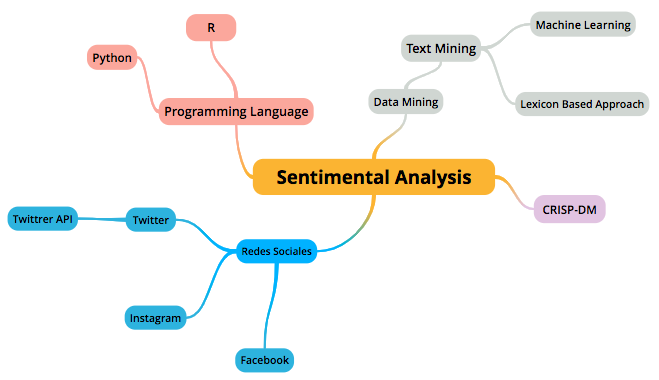
\includegraphics[scale=0.4]{../chapters/img/Ch04_MM.PNG}
\caption{Mapa Mental}
\end{figure}
\end{frame}


%
\begin{frame}
\frametitle{Metodolog\'ia}
\begin{figure}[H]
\centering
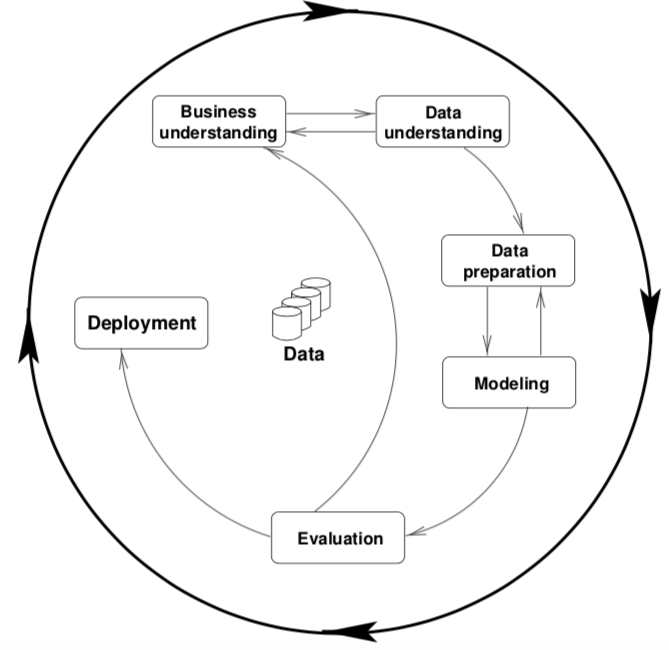
\includegraphics[scale=0.25]{../chapters/img/Ch06_CRISP.PNG}
\caption{Fase del proceso de modelo CRISP-DM}
\end{figure}
\end{frame}



%
\begin{frame}
\frametitle{Cronograma}
\begin{figure}[H]
\centering
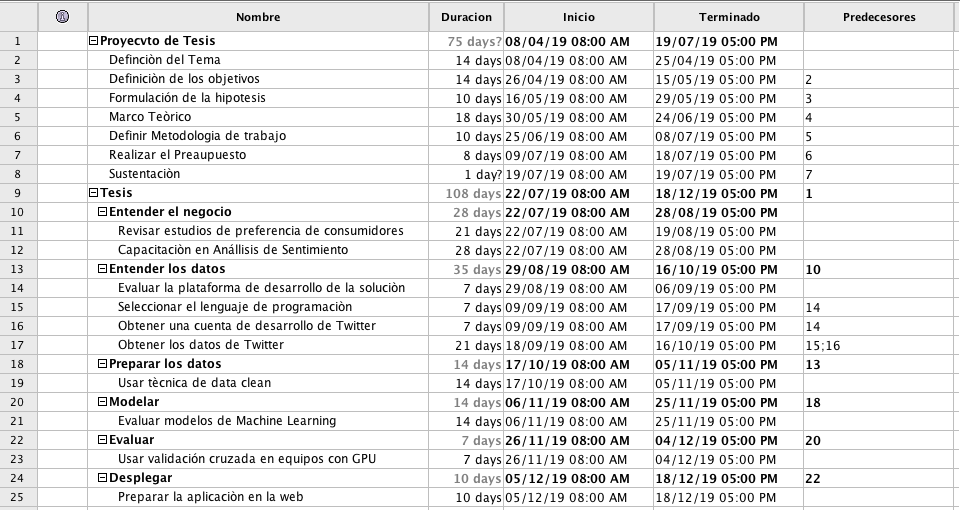
\includegraphics[scale=0.3]{../chapters/img/Ch07_schedule.PNG}
\caption{Cronograma del Proyecto de Tesis y la Tesis}
\end{figure}
\end{frame}

\end{document}